\documentclass[11pt]{article}
\usepackage[margin=1in, head=1in]{geometry}
\usepackage{amsmath, amssymb, amsthm}
\usepackage{fancyhdr}
\usepackage{graphicx}
\usepackage{pgfplots}
\usepackage{verbatim}

%\usepackage{pdfsync}
\addtolength{\textwidth}{.5in}
\addtolength{\leftmargin}{-1in}
\addtolength{\textheight}{.5in}
\addtolength{\topmargin}{-0.5in}

%\pagestyle{fancy}
%\lhead{MATH 200X }
%\chead{Fall 2007}
%\rhead{FINAL EXAM}
%\lfoot{}
%\cfoot{\thepage}
%\rfoot{}

\setcounter{secnumdepth}{0}
\newcommand{\R}{\mathbb{R}}
\newcommand{\N}{\mathbb{N}}
\newcommand{\Z}{\mathbb{Z}}
\newcommand{\clm}{\par\textit{Claim:}\par}
\newcommand{\diam}{\mathrm{diam}}
\newcommand{\sect}{\textsection}

\parindent=0in
\parskip=0.5\baselineskip

\begin{document}
\newgeometry{top=3in}
\begin{center}
\vspace{2in}

\huge{Math 156 PRECALCULUS \\
Fall 2015}

\vfill

\huge{\bf{Quiz 4 -- Version One}}\vspace{0.5in}

\large{Thursday, October 1, 2015}\\

\vfill


{\huge{Name:{\underline{\hspace{2in}}}}}
\vfill
This quiz has 5 problems worth a total of 30 points. It is TWO SIDED. 
\vfill
\end{center}
\newpage
\restoregeometry
\begin{enumerate}
%2.2.20%%
\item (5 points) For the function $g(x)=\sqrt{x+3}$, (i) make a table of values and then (ii) sketch the graph on the axes below.
 \begin{flushright} \begin{tikzpicture}
\draw[->, thick] (-3,0) -- (4,0)node [pos=1, below] {$x$};
\draw[->, thick] (0,-3) -- (0,4) node [pos=1, left] {$y$};
\end{tikzpicture}\end{flushright}

%2.2.45
\item (5 points) Sketch a graph of the piecewise defined function:\\
 $f(x) =
  \begin{cases} 
      \hfill 4    \hfill & \text{ if $x<-2$} \\
      \hfill x^2    \hfill & \text{ if $-2\leq x<2$}\\
      \hfill x-1 \hfill & \text{ if $2\leq x$} \\
  \end{cases}$
  
\vspace{-1in}
\begin{flushright} 
\begin{tikzpicture}
\draw[->, thick] (-3,0) -- (4,0)node [pos=1, below] {$x$};
\draw[->, thick] (0,-3) -- (0,4) node [pos=1, left] {$y$};
\end{tikzpicture}
\end{flushright}

%2.3.7, 2.3.13, 2.3.33
\item (10 points) Answer the questions using the graph of $f(x)$ shown below.\\

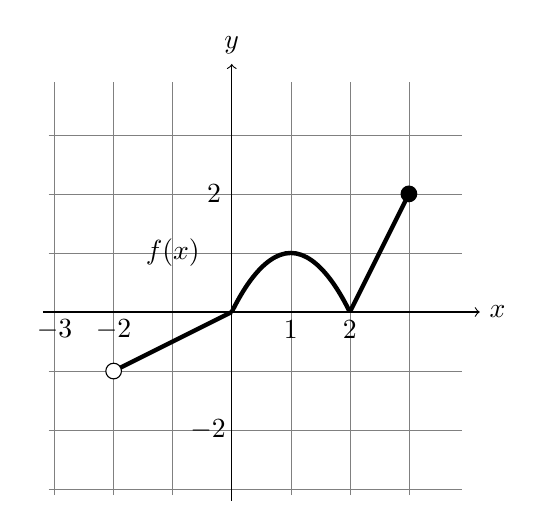
\begin{tikzpicture}[domain=-3:4, scale=.75]
    \draw[very thin,color=gray] (-3.1,-3.1) grid (3.9,3.9);
    \draw[->] (-3.2,0) -- (4.2,0) node[right] {$x$};
    \draw[->] (0,-3.2) -- (0,4.2) node[above] {$y$};
    \draw[ ultra thick] (-2,-1) -- (0,0);
    \draw[ultra thick] (0,0) parabola bend (1,1) (2,0);
    \draw[ultra thick] (2,0) -- (3,2);
    \node[circle,draw=black,fill=white, inner sep=2pt] at (-2,-1){};
    \node[circle,draw=black,fill=black, inner sep=2pt] at (3,2){};
    \node at (-1,1){$f(x)$};
    \node at (-2,-.3){$-2$};\node at (-3,-.3){$-3$};\node at (1,-.3){$1$};\node at (2,-.3){$2$};
    \node at (-.3,2){$2$};\node at (-.4,-2){$-2$};
    \end{tikzpicture}
    
\vspace{-2.5in}
\begin{flushright}{domain of $f(x)$ is: \underline{\hspace{2in}}}\end{flushright}
\begin{flushright}{range of $f(x)$ is: \underline{\hspace{2in}}}\end{flushright}
\begin{flushright}{$f(1)= $\underline{\hspace{2in}}}\end{flushright}
\begin{flushright}{Solve $f(x)=0:$\underline{\hspace{2in}}}\end{flushright}

\hspace{3.25in} Give the intervals on which
\begin{flushright}{ $f(x)$ is increasing.\underline{\hspace{2in}}}\end{flushright}

\newpage
%2.4.21
\item (4 points) For $f(x)=\frac{1}{x},$  find the {\bf{net change}} from $x=2$ to $x=2+h,$ and simplify your answer. You must show your work to receive credit.

\begin{flushright}{ Answer:\underline{\hspace{2in}}}\end{flushright}
\vfill

%2,4.24
\item (6 points) For $f(x)=1-3x^2,$ find the {\bf{average rate of change}} from $x=a$ to $x=a+h$ and simplify your answer. You must show your work to receive credit.

\begin{flushright}{ Answer:\underline{\hspace{2in}}}\end{flushright}
\vfill



\end{enumerate}
\end{document}

%1.11.38
\item (6 points) Use the graphs below to solve the inequality $3x+10 > 6x^2-x^3.$\\
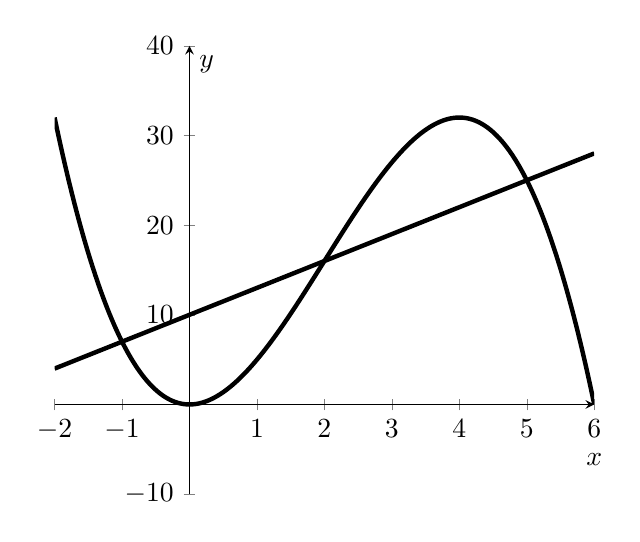
\begin{tikzpicture}[scale=1]
\begin{axis}[
        axis x line=middle, 
        axis y line=middle, 
        ymax=40, 
        ymin=-10,
        ylabel=$y$, 
        xtick={-2,-1,1,2,3,4,5,6},
        x label style={at={(current axis.right of origin)},anchor=north, below=5mm},
         xlabel=$x$,
        %x label style={at={(axis description cs:4,-1)},anchor=north},
        ]
    \addplot[domain=-2:6, samples=400, black, ultra thick]  {3*x+10};
    \addplot[domain=-2:6, samples=400, black, ultra thick]  {6*x^2-x^3};
\end{axis}
\end{tikzpicture}
\begin{flushright}{Answer: \underline{\hspace{2in}}}\end{flushright}
